In this section we review the necessary theoretical background for setting up and understanding the MOT.

\subsection{Laser Cooling}
The general principle of laser cooling can be understood by considering atoms with two possible values of total angular momentum, i.e.\ $j=0$ and $j=1$. Both states are seperated by an energy gap $\Delta E$.
\begin{figure}[h]
  \centering
  \begin{tikzpicture}
    \draw (0,0)--(5,0) node[right] {$j=0$};
    \draw (0,2)--(5,2) node[right] {$j=1$};
    \draw [<->] (1,0.1)--(1,1.9);
    \draw (1.4,1) node {$\Delta E$};
  \end{tikzpicture}
  \caption{Two-state system as a model for atoms.}
  \label{fig:two_state}
\end{figure}

Aligning a laser beam with frequency $\omega$ on the atom(s), the cross section $\sigma(\omega)$ for the absorption of photons can be modelled by a Lorentzian
\begin{align*}
  \sigma(\omega) =\alpha \cdot \frac{1}{1+\beta (\omega-\omega_0)^2}
\end{align*}
with some constants $\alpha,\beta >0$ and the resonance frequency $\omega_0=\Delta E/\hbar$. For laser cooling one uses a laser with a frequency $\omega_\mathrm{L}$ smaller than the resonance frequency, i.e.\ $\omega_\mathrm{L} < \omega_0$ (see figure \ref{fig:detuning}). 
\begin{figure}[h]
  \centering
  \begin{tikzpicture}
    \draw [->] (0,0)--(0,3) node [left] {$\sigma$};
    \draw [->] (0,0)--(5,0) node [below] {$\omega$};
    \draw[domain=0:5, smooth, variable=\x, smaples=1000] plot ({\x},{3/(1+(\x-2.5)^2)});
    \draw [dotted] (2.5,3)--(2.5,0) node [below] {$\omega_0$};
    \draw [dotted] (1.7,1.83)--(1.7,0) node [below] {$\omega_\mathrm{L}$};
  \end{tikzpicture}
  \caption{Schematic graph of the cross section.}
  \label{fig:detuning}
\end{figure}

If the atom moves with the velocity $v$ towards the laser the laserfrequency gets blueshifted for the atom
\begin{align*}
  \omega_\mathrm{L}' = \omega_\mathrm{L} \left(1+\frac{v}{c}\right).
\end{align*}
This means that (if $v$ is not to high) the atom will absorb more photons since $\omega_\mathrm{L}<\omega_0$. Since the direction of photons being emitted spontaneously is random the atom does not get a netto momentum from the emission of many photons. However, the atom gains momentum against the direction of movement from the absorption of the photons. This momentum slows the atom down. In order not to get accelerated in the opposite direction after the slowing down one uses a second laser with the same frequency aligned from the opposite direction. In three dimensions one thus uses six laser beams on three orthogonal axes.

\subsection{Trapping Atoms}
In every spontaneous emmission the atom gains momentum in a random direction. This means that the atom will not be slowed down completely but performs a random walk with the average velocity being zero. During this random walk the atom will leave the focus of the laser beams and hence diffuse out of the cooling zone. To prevent the atoms from diffusing one needs a position dependent force. This can be achieved by the use of an inhomogeneous magnetic field. For the explanation of the effect we consider cooling in one dimension with an magnetic field depending on the position $x$ as
\begin{align*}
  B=B_0 \frac{x}{x_o}
\end{align*}
with some constants $B_0,x_0>0$. We assume that (compare to the normal Zeeman effect) the energy levels get shifted by 
\begin{align*}
  E_{j,m_j} \mapsto E_{j,m_j}+\mu B m_j
\end{align*}
with the constant magnetic moment $\mu$. This change breaks the degeneracy of the three $j=1$ states and splits the energy differences $\Delta E$ (and thus the resonance frequency $\omega_0$) into three different energies. The position dependence of the splitting can be used to get a position dependent force by using $\sigma^\pm$-polarized laser beams. $\sigma^+$- ($\sigma^-$-) polarized light can only be absorbed by the transition $m_j=0 \mapsto 1$ ($m_j=0 \mapsto -1$). With the setup of figure \ref{fig:trap} we get a force pushing the atoms to the point $x=0$.
\begin{figure}[h]
  \centering
  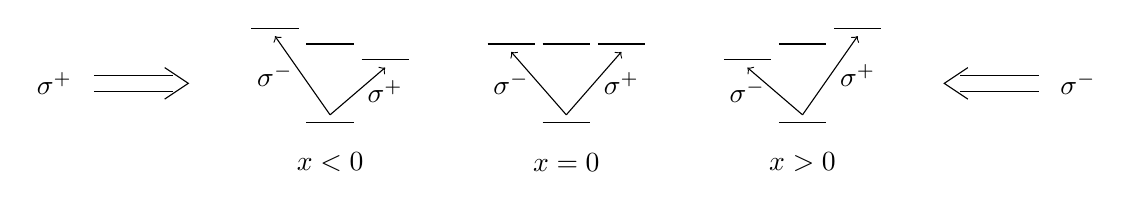
\begin{tikzpicture}
    \draw (-0.3,0)--(0.3,0);
    \draw (-0.3,1)--(0.3,1);
    \draw (-0.3-0.7,1)--(0.3-0.7,1);
    \draw (-0.3+0.7,1)--(0.3+0.7,1);
    \draw [->] (0,0.1)--(0.7,0.9); 
    \draw (0.7,0.5) node {$\sigma^+$};
    \draw [->] (0,0.1)--(-0.7,0.9); 
    \draw (-0.7,0.5) node {$\sigma^-$};
    \draw (0,-0.5) node {$x=0$}; 

    \draw (-0.3+3,0)--(0.3+3,0);
    \draw (-0.3+3,1)--(0.3+3,1);
    \draw (-0.3-0.7+3,1-0.2)--(0.3-0.7+3,1-0.2);
    \draw (-0.3+0.7+3,1+0.2)--(0.3+0.7+3,1+0.2);
    \draw [->] (0+3,0.1)--(0.7+3,0.9+0.2); 
    \draw (0.7+3,0.5+0.1) node {$\sigma^+$};
    \draw [->] (0+3,0.1)--(-0.7+3,0.9-0.2); 
    \draw (-0.7+3,0.5-0.1) node {$\sigma^-$};
    \draw (0+3,-0.5) node {$x>0$}; 

    \draw (-0.3-3,0)--(0.3-3,0);
    \draw (-0.3-3,1)--(0.3-3,1);
    \draw (-0.3-0.7-3,1+0.2)--(0.3-0.7-3,1+0.2);
    \draw (-0.3+0.7-3,1-0.2)--(0.3+0.7-3,1-0.2);
    \draw [->] (0-3,0.1)--(0.7-3,0.9-0.2); 
    \draw (0.7-3,0.5-0.1) node {$\sigma^+$};
    \draw [->] (0-3,0.1)--(-0.7-3,0.9+0.2); 
    \draw (-0.7-3,0.5+0.1) node {$\sigma^-$};
    \draw (0-3,-0.5) node {$x<0$}; 

    \draw (-6,0.6)--(-5,0.6);
    \draw (6,0.6)--(5,0.6);
    \draw (-6,0.4)--(-5,0.4);
    \draw (6,0.4)--(5,0.4);
    \draw (-5.1,0.7)--(-4.8,0.5)--(-5.1,0.3);
    \draw (5.1,0.7)--(4.8,0.5)--(5.1,0.3);
    \draw (-6.5,0.5) node {$\sigma^+$};
    \draw (6.5,0.5) node {$\sigma^-$};
  \end{tikzpicture}
  \caption{Position dependent force induced by inhomogeneous magnetic field and polarized beams. The three upper levels correspond to $m_j=-1,0,1$.}
  \label{fig:trap}
\end{figure}

In three dimensions the same effect is achieved by using an quadrupole field generated by an anti-Helmholtz configuration of coils.

\subsection{Trapping Rubidium Atoms}
The atoms that we want to cool down in this experiments are $^{85}$Rb atoms. The level structure can be found in figure \ref{fig:level_structure}. \newpage
\begin{figure}[h]
  \centering
  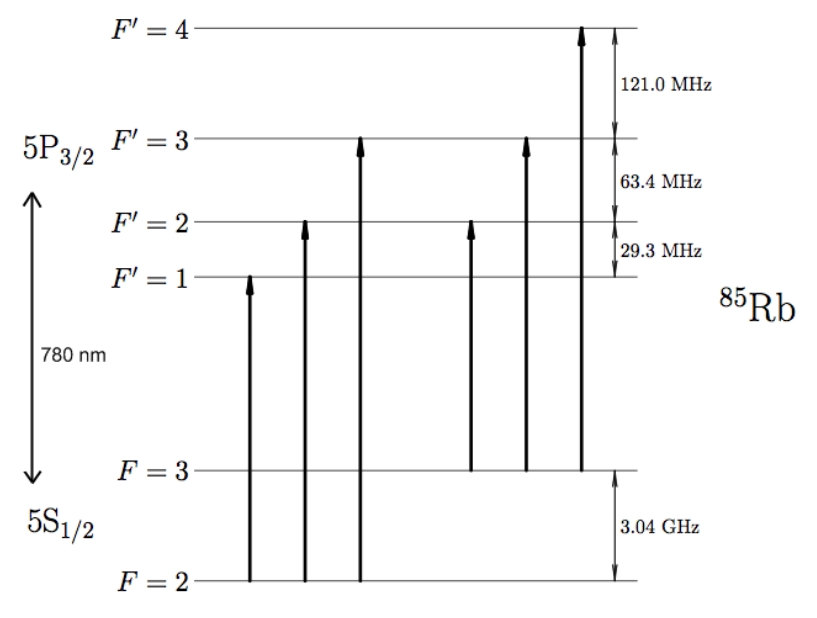
\includegraphics[width=0.5\textwidth]{figures/level_structure.png}
  \caption{Level structure of $^{85}$Rb.}
  \label{fig:level_structure}
\end{figure}

For the cooling we use the transition $F=3 \mapsto F'=4$. Due to rare excitations from $F=3$ to $F'=2,3$ the atoms can decay into the state $F=2$ and are then no longer available for the cooling. To get these atoms back into the cooling scheme one uses a pump laser which pumps atoms from $F=2$ to $F'=3$. 

\subsection{Polarization Spectroscopy}
For the MOT to work we need two lasers (the cooling laser and the pump laser) at two constant frequencies. In this experiment diode lasers are used. The laser diode emitts laser light of different frequencies. To filter out one frequency one uses a grating with an adjustable angle. For different angles, different frequencies are filtered out. Due to fluctuations of the temperature and the electron density the filtered out frequency is not stable. To adjust this one uses a Piezo element which adjusts the angle of the grating if the frequency changes. The error signal for the Piezo is obtained by the use of polarization spectroscopy. For the explanation of this technique we start describing the saturation spectroscopy.\\

For saturation spectroscopy the laser beam is divided into two beams. One high intensity pump beam and one low intensity test beam. Both beams are aligned on a probe ($^{85}$Rb in our case) from approximately opposite directions. The transmission of the test beam is measured with a photo diode. If the lasers are in resonance with a transition of the atoms, the pump beam will pump the atoms in the excited state. The atoms can then no longer absorb the photons of the test beam which results in a higher transmission, the so called Lamb dip (figure \ref{fig:lamb_dip}). As this mostly concerns atoms which do not move in the direction of the beams, this procedure is also called Doppler-free spectroscopy.
\begin{figure}[h]
  \centering
  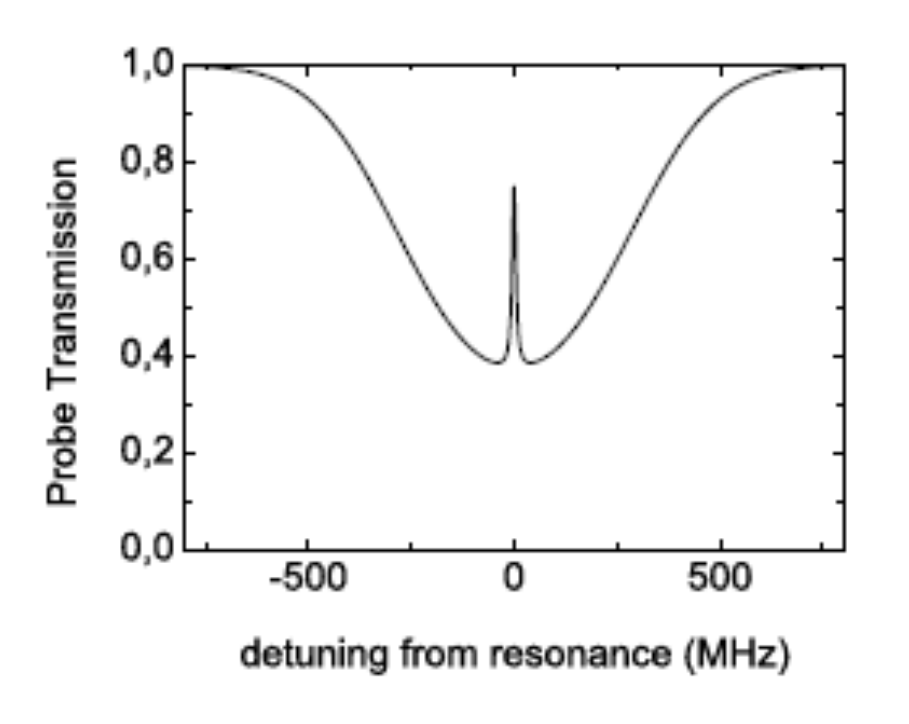
\includegraphics[width=0.4\textwidth]{figures/lamb_dip.png}
  \caption{Lamb dip from saturation spectroscopy.}
  \label{fig:lamb_dip}
\end{figure}

For the polarisation spectroscopy one uses the same setup as in the saturation spectroscopy with the difference, that the pump beam is either $\sigma^+$- or $\sigma^-$-polarized. This results in an anisotropic population of the different $m_F$ states which makes the probe birefringent. As a result a linear polarized test beam then gets split into two components. One measures both transmission signals and subtracts them. The final signal has the form of the derivative of the transmission signal in figure \ref{fig:lamb_dip}. This signal can be used to lock the laser, i.e.\ it is used as the error signal for the Piezo.
